\documentclass[Arkitektur/System_main.tex]{subfiles}
\begin{document}
\section{Deployment View}
\begin{figure}
    \centering
    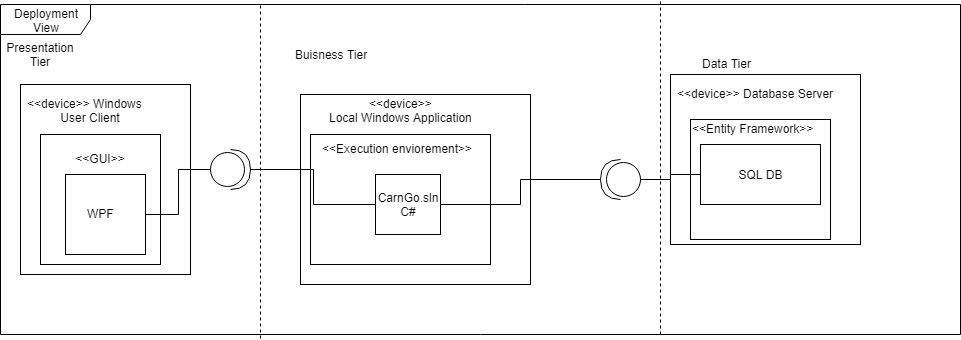
\includegraphics[width=\linewidth]{Arkitektur/4+1View/Graphics/DeploymentDiagram.png}
    \caption{Deployment View}
\end{figure}

For oven ses der et diagram der fremviser den fysiske forbindelse mellem vores program og de forskellige lag som applikationen operer i. 

Disse lag kan opdeles i tre dele "Præsentation tier" som fremviser de dele af vores system som brugeren interagerer med. Den første del kan vi se at vores "Windows User Client" som repræsenterer selve applikationen som vores brugere benytter. Inde i den kan vi så se en box der indikerer hvordan denne User client er sat op. 

I vores applikation specifikt bruger vi WPF til at kode brugergrænsefladen. Vi kan her se at WPF koden her er forbundet til vores C\# kode i det næste lager. 

Det næste lager er vores "Buisness Layer" som er den del af vores applikation der tager informationen fra brugergrænsefladen og behandler den information for at så sende information tilbage til WPF koden sådan at brugeren kan se hvad der sker når de interagerer med GUI'en. 

Dette er så den lokale Windows applikation der findes på brugerens PC, som indeholder vores "Execution Enviorement" der repræsenterer den del af vores applikation der udfører det funktionelle. 

Buisness Tier er derfra forbundet til et Data Tier, som er den del af vores applikation der indeholder en database der gemmer på dataen vi modtager fra brugeren fra GUI'en igennem vores CarNGo.sln fil. I vores applikation har vi valgt at benytte en SQL server efter noget diskussion om hvor hvidt vi ville bruge noget andet men besluttede at bruge en SQL. 

Vi bruger Entity Framework som et mellemled mellem vores database og resten af koden for at vi kan tage informationen fra C\# kode og sætte det ind i et SQL miljø. 
\end{document}